\documentclass[12pt, a4paper]{report}
\usepackage[utf8x]{inputenc}
\usepackage[T1]{fontenc}
\usepackage[hungarian]{babel}
\usepackage{amsmath}
\usepackage{amsfonts}
\usepackage{amssymb}
\usepackage{amsthm}
\usepackage{ccfonts}
\usepackage[euler-digits,euler-hat-accent]{eulervm}
\usepackage{graphicx}
\usepackage{ae}
\usepackage[margin=2cm]{geometry}
\usepackage{hyperref}
\usepackage{minted}
\usepackage[parfill]{parskip}
\usepackage{enumitem}

\makeatletter

\graphicspath{ {./images/} }

\newcommand{\f}[1]{\texttt{#1}}
\newcommand{\ff}[1]{\textbf{\texttt{#1}}}
\newcommand{\bb}[1]{\textbf{#1}}

\newminted[mmcode]{"../pygments/MetaLexer.py":MetaLexer -x}{tabsize=2,fontsize=\footnotesize,baselinestretch=0.7,linenos=false,frame=single,breaklines=true,breakanywhere=true,style=sb}
\newminted{csharp}{tabsize=2,fontsize=\footnotesize,baselinestretch=0.7,linenos=false,frame=single,breaklines=true,breakanywhere=true,style=sb}

\setitemize{noitemsep,topsep=0pt,parsep=0pt,partopsep=0pt}


% Title Page
\title{DSL alapfogalmak}
\author{Dr. Simon Balázs}
\date{\today}


\begin{document}
\maketitle

\tableofcontents

\chapter{Bevezetés}

Ez a dokumentum a szakterület-specifikus nyelvekkel és a fordítással kapcsolatos alapfogalmakat definiálja.

Az első fejezet a modellvezérelt architektúrát, a metamodellezést és a szakterület-specifikus nyelveket mutatja be.

A második fejezet a fordítás típusait és fázisait ismerteti.


\chapter{Szakterület-specifikus nyelvek (DSL)}

A modellvezérelt architektúrát (\bb{Model Driven Architecture, MDA}) \cite{Mel04} \cite{Fra02} az Object Management Group (OMG) definiálta. Egy \bb{modell} olyan elemek halmaza, amelyek valamilyen fizikai, absztrakt vagy hipotetikus világot írnak le. A modellezéshez absztrakcióra és osztályozásra van szükség. Az \bb{absztrakció} azt jelenti, hogy az adott kontextusban lényegtelen információkat elhanyagoljuk. Az \bb{osztályozás} azt jelenti, hogy a vizsgált dolgokat közös tulajdonságaik és viselkedésük alapján csoportosítjuk. Az MDA szerint különböző modellek különböző absztrakciós szinteken jelenhetnek meg, és ezeket a modelleket össze is kapcsolhatjuk, hogy egy működő implementációt kapjunk. Egyes modellek függetlenek a megcélzott szoftveres platformtól, más modellek pedig specifikusak arra. Egy \bb{platform} egy futtatási környezetet definiál modellek egy halmazára. Platformok lehetnek a különböző keretrendszerek (pl. Java vagy .NET), operációs rendszerek (pl. Windows vagy Linux), adatbázismotorok (pl. MySQL vagy Oracle DB), és más specifikus szoftverrendszerek.

A modelleket modellező nyelvek írják le. Az OMG által létrehozott szabványos modellező nyelv a Unified Modeling Language (UML). Ez egy \bb{általános célú modellező nyelv} (General Purpose Language, GPL), azaz nincs hozzákötve egyetlen alkalmazási területhez sem. Az absztrakciós szintje közel áll a hagyományos általános célú programozási nyelvekhez (pl. Java, C\# és C++), amelyek széles kifejezőerővel rendelkeznek, hiszen Turing-teljesek. Egy \bb{szakterület-specifikus nyelv (Domain Specific Language, DSL)} \cite{Voe13} \cite{Fow10} olyan progamozási nyelv, amely korlátozott kifejezőerővel rendelkezik, de egy adott alkalmazási területre fókuszál. Így egy teljes szoftvert nem lehet egy DSL segítségével megvalósítani, egy DSL mindössze a szoftver egy adott aspektusának leírására alkalmas. Egy DSL fókuszáltsága az, ami miatt megéri azt használni, mert így az adott alkalmazási terület fogalmaival tudunk dolgozni. Az UML szabványban a profilok segítségével az UML fogalomrendszere is kiterjeszthető szakterület-specifikus elemekkel, de ezek használati lehetőségei korlátozottak és kényelmetlenek lehetnek \cite{Voe13}.

Egy DSL lehet belső vagy külső. A \bb{belső DSL} egy általános célú programnyelv egyes elemeinek speciális módon történő felhasználását jelenti. Egy belső DSL-ben leírt szkript valójában a befoglaló programnyelv egy részhalmazának használatát jelenti. A belső DSL előnye, hogy nem kell hozzá új programnyelvet megtanulni, és nem kell hozzá fordítót írni. Hátránya azonban az, hogy szintaktikáját korlátozza az őt befoglaló általános nyelv szintaktikája, nem lehet minden szakterületi szabályt fordítási időben ellenőrizni, és nem lehet garantálni, hogy az általános nyelv előírt részhalmazát használjuk csak. További hátrány, hogy csak az általános nyelven belül használható, nem lehet más módon feldolgozni. Egy külső DSL az egy önálló nyelv, amely független az alkalmazás implementációs nyelvétől. A \bb{külső DSL} általában speciális szintaxissal rendelkezik, de lehet egy létező szintaxist is DSL-ként használni (pl. XML-t). A külső DSL előnye, hogy a szakterület fogalmai nyelvi elemként jelennek meg, a szintaktika szabadon alakítható a saját ízlésünknek megfelelően, gazdag nyelvi ellenőrzéseket lehet rá írni, többfajta célnyelvre is fordítható és többféle értelmező is készíthető hozzá (pl. végrehajtható C kód, tesztesetek, szimuláció, stb.). Hátránya, hogy egy új programnyelvet kell alkotni, amit meg is kell tanulni a felhasználóknak, és saját fordítót és értelmezőt is kell hozzá írni.

Metamodellnek hívjuk egy modell modellezési nyelvét. A metamodellezésnek több szintje is van, hiszen egy metamodell elemeit is le kell tudni írni valahogy:

\begin{center}\includegraphics[trim=0 0 0 0,clip,width=\textwidth,page=13]{Images.pdf}\end{center}

A \bb{metamodell} definiálja a modell elemeinek struktúráját, szemantikáját és kényszereit. Például az UML modellek elemeit az UML metamodell definiálja. Ilyen elemek a Class, Property, Association, State stb. Az UML metamodell ezen elemek jelentését is megadja. Például a Type elem értékek egy halmazát reprezentálja. Az UML metamodell az elemekre vonatkozó kényszereket is leír. Például egy kompozícióval tartalmazott elemnek nem lehet egynél több tartalmazója. Az UML metamodellt a MOF meta-metamodell írja le, az UML metamodell pedig a MOF meta-metamodell egy példánya. A MOF elég általános ahhoz, hogy az UML-en kívül más modellezési nyelveket, például különböző DSL-eket is le tudjon írni, de ahhoz is, hogy önmagát leírja. Így a MOF felett már nem kell újabb metamodell nyelvet definiálni. A metamodellezésnek köszönhetően az MDA elvei DSL-ekre is alkalmazhatók, így jutunk el a szakterület-specifikus modellezéshez (\bb{Domain Specific Modeling, DSM}) \cite{Kel08}. A DSM tovább növelheti a fejlesztés produktivitását az eredeti UML alapú MDA megközelítéshez képest, mivel a speciális DSL-ek magasabb absztrakciós szintűek lehetnek, mint maga az UML \cite{Ste09} \cite{Met18}.

Egy metamodell írja le modellek a strukturális és viselkedésbeli aspektusait, de azt nem adja meg, hogyan kell ezeket a modelleket grafikusan vagy szövegesen reprezentálni, vagy netán szerkeszteni. A \bb{konkrét szintaxis} az, ami definiálja a grafikus, szöveges, táblázatos, szimbolikus vagy egyéb reprezentációját egy modellnek. A konkrét szintaxis adja meg azt a jelölésrendszert, amely segítségével a felhasználó definiálni és szerkeszteni tudja a modellt. Az \bb{absztrakt szintaxis} adja meg a modell szemantikai lényegét, vagyis jelentését. Az absztrakt szintaxis nem tartalmazza a jelölésrendszer részleteit, mint a színek, pozíciók, szimbólumok és kulcszavak. Így a metamodell tekinthető az absztrakt szintaxisnak. A modell elemzése és feldolgozása az absztrakt szintaxison keresztül történik, és a kódgenerálás is az absztrakt szintasis segítségével valósul meg.

A \bb{szöveges konkrét szintaxis} előnye a grafikus konkrét szintaxishoz képest, hogy könnyebb a kódot írni és szerkeszteni, mint grafikus elemeket megrajzolni. A szöveges szintaxisnak nagyobb kifejezőereje is van és könnyebb verziókezelni is. A \bb{grafikus konkrét szintaxis} előnye az, hogy szemléletesebb, így könnyebb olvasni, mint a szöveges szintaxist.

\chapter{Fordítás}

A fejlesztők különböző programnyelveket használnak a számítógép működésének vezérlésére. A legelterjedtebb programnyelvek (pl. C\#, Java, C++, Python) \bb{általános célú nyelvek}, amelyek Turing-teljesek, így tetszőleges algoritmus megfogalmazható a segítségükkel. Hasznosak lehetnek azonban a speciális célra kifejlesztett saját \bb{szakterület-specifikus nyelvek} (Domain Specific Language, DSL) is, amelyek fogalomrendszere közelebb áll a saját fogalmainkhoz, ezáltal tömörebben és érthetőbben megfogalmazhatók a szakterület egyes problémáira adott megoldások. Az ilyen szakterület-specifikus nyelvek nem feltétlenül Turing-teljesek, és sokszor az a céljuk, hogy átfordítsuk őket általános programnyelvekre.

A \bb{fordítás célja} a szöveges forrásnyelv átvitele a célnyelvre a \bb{jelentés megtartásával}. A forrás- és célnyelv lehetnek azonosak, de a célnyelv lehet akár a számítógép által értelmezhető is.

Egy programnyelv jelentését a nyelv specifikációja fogalmazza meg. A modern általános célú nyelvek esetén (pl. C\#, Java, Python) a jelentés erősen összefügg a kód struktúrájával. Az adattípusok és a vezérlőszerkezetek is egymásba ágyazott struktúrát követnek.

A fordítás lehetséges típusai: interpretálás, előfordítás, futási-idejű fordítás, teljes fordítás és makrók helyettesítése. Az \bb{interpretálás} során egyenként értelmezzük és hajtjuk végre az egyes kifejezéseket és utasításokat. Tipikusan ilyenek a parancsértelmezők (pl. bash, Windows parancssor), illetve az interpretált programnyelvek (pl. JavaScript, Python). Az \bb{előfordítás} célja egy előzetes hibaellenőrzés után az interpreter által könnyen értelmezhető nyelvre (köztes kódra) történő fordítás. Így működik a Java fordító, ahol a köztes kód a Java bájtkód, az interpreter pedig a Java virtuális gép (JVM). A \bb{futási-idejű fordítás} során a forráskódból előállított köztes kód továbbfordítása történik gépi kódra. Ezt teszi például a .NET keretrendszer JIT (Just-In-Time) fordítója. A \bb{teljes fordítás} a közvetlen gépi kódra történő fordítást jelenti. Ez a korai általános célú nyelvek (pl. C, C++, Pascal) működési módja. A makróhelyettesítésnél a forrás és a célnyelv megegyeznek, a makrók csak helyettesítési szabályokat definiálnak. Ilyen a C és C++ makró megoldása.

Bármilyen jellegű forrásnyelvről is legyen szó, a nyelvet értelmezni tudó fordítóprogramok általában hasonló módon működnek. A fordító két részre bontható: a front-end és a back-end. A \bb{front-end} feladata a programnyelv szöveges tartalmának feldolgozása, abból a jelentés kinyerése, és az előforduló hibák jelzése. Amennyiben nincs hiba, a front-end egy olyan modellt épít a memóriában, amelyet a \bb{back-end} le tud képezni a célnyelvre. A back-end tipikusan már nem foglalkozik hibakereséssel, mert feltételezzük, hogy a front-end által épített modell helyesen leképezhető a célnyelvre.

A \bb{fordítás fázisait} az alábbi ábra foglalja össze:

\begin{center}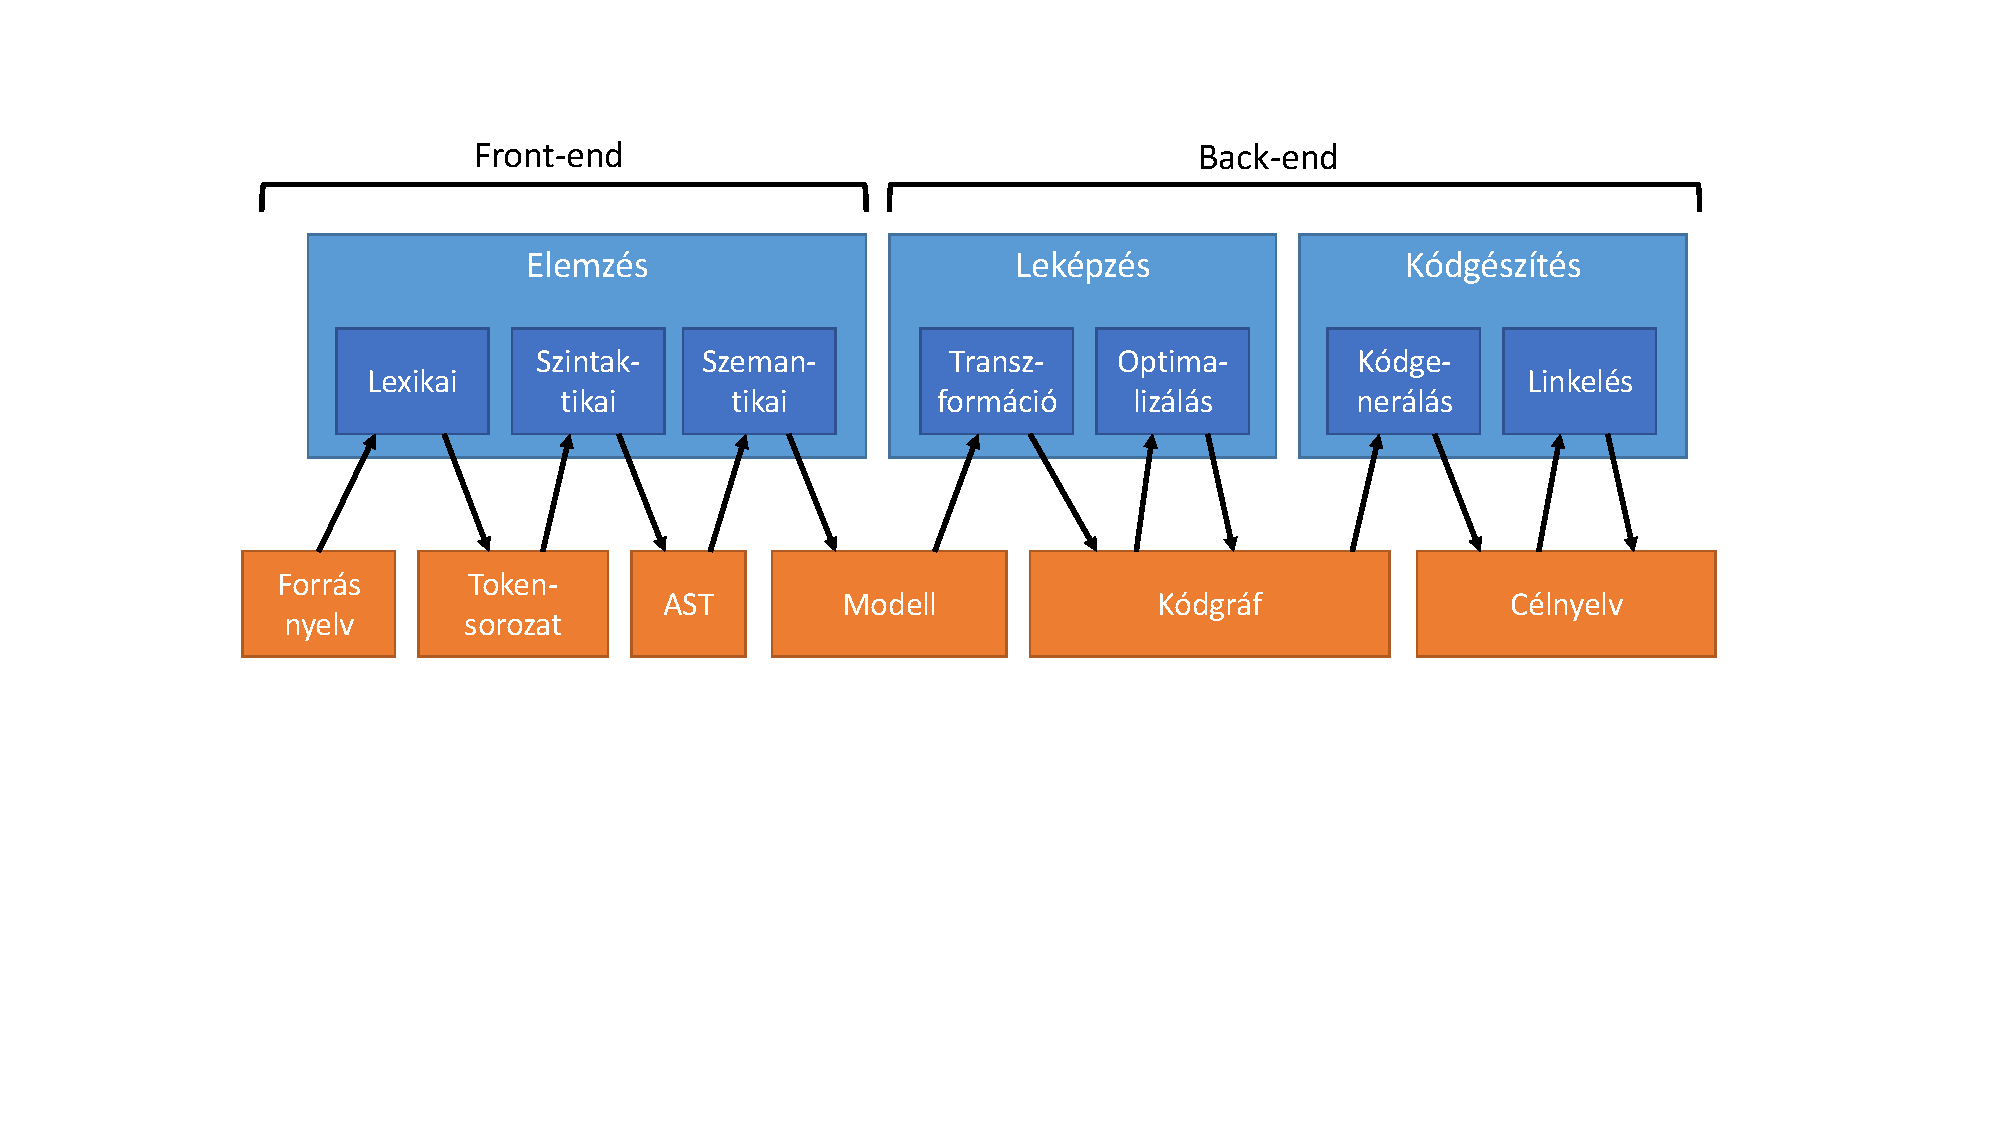
\includegraphics[trim=110 220 120 60,clip,width=\textwidth,page=1]{Images.pdf}\end{center}

A \bb{lexikai elemzés} feladata a forráskód feldarabolása jelentéssel bíró egységekre (\bb{token}-ekre). A lexikai elemzés általában figyelmen kívül hagyja a felesleges karaktereket (pl. szóközök, üres sorok és kommentek). A modern programnyelvek (pl. C\#, Java, Python) általában úgy lettek megtervezve, hogy a lexikai elemzés független a későbbi fázisoktól, így az hatékonyan, véges automaták segítségével megvalósítható. A \bb{lexer} (lexikai elemző) definiálása reguláris kifejezésekkel történik. A reguláris kifejezések véges automatákká alakíthatók, és ezek a véges automaták ismerik fel az egyes tokeneket. Ilyen tokenek tipikusan a white-space (szóköz, új sor), a kommentek, a kulcsszavak (pl. C\#-ban az if, class, private, stb.), a számok, az azonosítók (pl. változónevek, saját típusnevek), stb. A lexer kimenete az így előálló tokenek sorozata. Amennyiben a programkód olyan karaktersorozatot tartalmaz, amely egyetlen tokenre sem illeszkedik, a lexer szintaktikai hibát jelez.

A \bb{szintaktikai elemzés} feladata a programkód fastruktúrájának felépítése. Ez a fastruktúra határozza meg a kód jelentését, pontosabban a jelentés egy részét. A \bb{parser} (szintaktikai elemző) definiálása kontextus-független (context-free, CF) nyelvtan segítségével történik. Az ilyen nyelvtanok kifejezőereje elég nagy a tipikus feladatokhoz, és mégis egyszerűen és gyorsan lehet őket elemezni. A parser bemenete a tokenek listája, kimenete a felépített fastruktúra, amelynek levelei a tokenek, csúcsai a CF nyelvtani szabályok példányai. Ha ez a fastruktúra tartalmaz minden tokent, akkor konkrét szintaxisfáról (Concrete Sytnax Tree, CST) beszélünk. Ha a fastruktúra csak a jelentés szempontjából releváns tokeneket tartalmazza, akkor absztrakt szintaxisfáról (Abstract Syntax Tree, AST) van szó.

A \bb{szemantikai elemzés} feladata a forráskód jelentésének teljes értelmezése. Például a parser által felépített fastruktúra még nem tartalmazza a típusinformációkat, és nem adja meg azt sem, hogy az egyes azonosítók (pl. függvény- és váltózónevek) felhasználása hogyan köthető az ő definíciójukhoz. A szemantikai elemzés fő feladata tehát a név- és típuselemzés, az azonosítók definíciójának és használatának összerendelése, és minden egyéb olyan konzisztencia-ellenőrzés, amelyet a programnyelv specifikációja előír (pl. típushelyesség ellenőrzése, interfészek és absztrakt függvények implementációja, stb.). A szemantikai elemzés bemenete a parser által felépített fastruktúra, kimenete pedig egy olyan modell, amit a back-end már értelmezni tud. Ez a modell lehet egyszerűen csak az AST szemantikai információkkal annotált változata is. A szemantikai elemzés az utolsó fázis, amely hibákat keres a kódban. Amennyiben ez a fázis hiba nélkül zárul, a back-end képes lesz a célnyelvre történő leképzést elvégezni.

A front-end feladatait a következő ábra szemlélteti:

\begin{center}\includegraphics[trim=120 120 120 110,clip,width=\textwidth,page=2]{Images.pdf}\end{center}

A \bb{back-end} abból a modellből indul ki, amelyet a front-end felépít. A back-end először egy platfromfüggetlen kódgráffá \bb{transzformálja} a modellt, amely később már minimális változtatásokkal a célnyelvre transzformálható. A platformfüggetlenség azért fontos, hogy többféle célnyelv is egyszerre támogatható legyen (pl. 32-bites és 64-bites architektúra). Ez a köztes \bb{kódgráf} a gépi fordítás esetén olyan elemi műveleteket tartalmazhat, mint például összeadás, kivonás, szorzás, osztás, érték kiírása egy adott memóriacímre, érték beolvasása egy adott memóriacímről, függvény meghívása adott memóriacímen, elágazások, ugró utasítások ciklusok implementálására stb. Az elemi műveletekből álló kódgráf lehetővé teszi, hogy a gráfon \bb{optimalizációt} tudjon végezni a back-end. Ilyen optimalizációk lehetnek gépi fordítás esetén az egymástól független műveletek sorrendjének átrendezése, konstans kifejezések kiértékelése, ciklusok magjának optimalizációja, jobb-rekurzív függvények ciklussá alakítása, stb.

Az optimalizált kódgráfból végül egy \bb{kódgenerátor} előállítja a célnyelvnek megfelelő reprezentációt. Gépi fordítás esetén a futtatható program előállításához össze kell \bb{linkelni} a binárisokat egyetlen állománnyá.

Ha nem gépi fordításról, hanem csak egyszerű kódgenerálásról van szó, a kódgenerátor közvetlenül a modellből is dolgozhat. Ilyenkor nincs szükség a köztes kódgráfra, és nincs szükség linkelésre sem.

\chapter{Összefoglalás}

Ez a dokumentum ismertette a metamodellezés, a szakterület-specifikus nyelvek (DSL) és a fordítás legfontosabb alapfogalmait.

\bibliographystyle{ieeetr}
\bibliography{references}

\end{document}          
